\documentclass[11pt]{amsart}

\usepackage{lmodern}
\usepackage{textcomp}
\usepackage[T1]{fontenc}
\usepackage{graphicx}
\usepackage{listings}
\usepackage{url}
\usepackage{tikz}
\usetikzlibrary{arrows}
\usepackage{xcolor}

\usepackage{studia}

%\lstset{
%  basicstyle=\ttfamily,
%  showstringspaces=false,
%  gobble=2
%}

\definecolor{codegreen}{rgb}{0,0.6,0}
\definecolor{codegray}{rgb}{0.2,0.2,0.2}
\definecolor{codeblue}{rgb}{0.0,0,0.62}
\definecolor{backcolour}{rgb}{0.95,0.95,0.92}

\lstdefinelanguage{scala}{
  morekeywords={abstract,case,catch,class,def,%
    do,else,extends,false,final,finally,%
    for,if,implicit,import,match,mixin,%
    new,null,object,override,package,%
    private,protected,requires,return,sealed,%
    super,this,throw,trait,true,try,%
    type,val,var,while,with,yield},
  otherkeywords={=>,<-,<\%,<:,>:,\#,@},
  sensitive=true,
  morecomment=[l]{//},
  morecomment=[n]{/*}{*/},
  morestring=[b]",
  morestring=[b]',
  morestring=[b]"""
}

\lstdefinestyle{mystyle}{
    language=scala,
    commentstyle=\color{codegreen}\itshape,
    keywordstyle=\color{codeblue}\bfseries,
    identifierstyle=\color{black},
    %numberstyle=\tiny\color{codegray},
    stringstyle=\color{black},
    basicstyle=\small\fontfamily{pcr}\selectfont\color{codeblue},
    %basicstyle=\small\ttfamily,
    breakatwhitespace=false,
    breaklines=true,
    captionpos=b,
    keepspaces=true,
    %numbers=left,                    
    %numbersep=5pt,                  
    showspaces=false,
    showstringspaces=false,
    showtabs=false,
    tabsize=2
}

\lstset{style=mystyle}

\tikzset{
  ->, >=stealth',
  level/.style={sibling distance = 2cm, level distance = 1cm},
  style = {text centered, inner sep=0pt},
  highlight/.style = {text=red}
}

\title{Compiler Front End Fusion: Undo Desugaring in Language
  Processing Tools}

\author{Art\'ur Po\'or}
\author{Tam\'as Kozsik}
\author{Melinda T\'oth}
\author{Istv\'an Boz\'o}

%\begin{keyword}
  % Parser \sep Abstract syntax tree \sep Compiler front end \sep Syntactic
  % sugar \sep Desugaring \sep Refactoring

  % \MSC 68N15 %%Programming languages
  % \sep 68N20 %%Compilers and interpreters
%\end{keyword}

\keywords{parser, abstract syntax tree, compiler front end, syntactic
  sugar, desugaring, refactoring}

\begin{document}

\lstMakeShortInline{@}

\begin{abstract}
  Compiler front ends often perform \emph{desugaring} on the source code
  while constructing the abstract syntax tree (AST).  A programming
  language processing tool (such as a refactoring tool) working with
  the desugared AST perceives the code at
  this abstract level, and loses information on the rich syntax used
  in the actual source code.  This paper discusses the concept of
  \emph{front end fusion}, a technique which may help language
  processing tools to retain the syntactic sugar information on the
  source code in the presence of desugaring compiler front ends. We
  propose a hybrid front end created from two separate front ends: one
  provided by the compiler, which offers type information, and
  another one, which provides the details of the concrete syntax used in the
  source code.
  As a case study, we show how to construct a hybrid front end in a
  language processing tool for the Scala programming language.
\end{abstract}

\maketitle

\section{Introduction}

Programming language processing tools provide invaluable help during
software development and maintenance. They can statically analyse source code for
debugging, code upgrade or grokking purposes, and they can perform
source code transformations and refactoring as well.
These tools typically need to be able to parse and pretty print
source code, and may also require semantic information, e.g. the type
of expressions and the result of name resolution.

There are two major approaches to implement language processing tools.
Firstly, the tool may have a custom lexer, parser, type checker,
static semantic analyser, and pretty printer built in, and tailored
for, the tool (\emph{standalone} approach).  Secondly, the
\emph{external} approach relies on some existing, widely-used compiler
infrastructure for the given programming language. However, as we
shall see, both approaches have disadvantages.

Older compilers provide no convenient ways to access the output of
the compiler front end. For example, earlier versions of GCC (before v4.5)
offer intermediate files for observing available information between different compilation
phases -- which is a rather inconvenient input to a language processing tool.
This is where the standalone approach may be needed: the tool needs to
re-implement (a part of) the compiler front end for the language. Obviously,
this is
quite expensive from the tool developer's point of view. Moreover,
this makes the tool more vulnerable against the evolution of the programming
language. 
Modern compilers such as Clang~\cite[p.~32]{llvm}, GHC~\cite{ghc-plugin} or
Scalac~\cite{programming-scala} provide
%application programming interface
APIs
to access (annotated) abstract syntax trees (AST) at different stages of
the compilation process. 
Annotated ASTs may convey not only syntactic information, but
semantic information (e.g. types) as well.
This turns out to be a useful input for a language processing tool
-- a clear benefit of the external approach.

Rich languages offer a great amount of syntactic sugar,
so that programmers can write terse, expressive, and easy-to-read code.
The syntactic sugar, however, is typically eliminated from the AST.
The compiler replaces certain fancy programming language constructs with
semantically equivalent simpler constructs (often referred to as \emph{core language}
constructs). This \emph{desugaring} process results in loss of information,
which can be a disadvantage of the external approach: the language processing
tool will be unable to reproduce the original, syntactically rich
source code.
Although syntactic sugar does not affect the meaning of a program (with respect
to core language constructs), it does have a significant impact on readability and
maintainability -- i.e. code quality. Therefore recovery of syntactic sugar in
a language processing tool is an essential issue.
For instance, we would like to observe the original, rich syntax, when the
tool communicates analysis results back to the programmer,
or pretty prints the code. 

As the main contribution, this paper proposes the concept of
\emph{front end fusion}: a technique to preserve syntactic sugar for a
programming language processing tool, if the external compiler
infrastructure used by the tool applies desugaring during the
construction of annotated abstract syntax trees. We propose a
\emph{hybrid front end}, a language processing tool front end, which
is the result of front end fusion: it is hybrid because it combines
external and standalone front ends. The presented approach performs
a fusion of a custom standalone parser and an external compiler
infrastructure when creating the hybrid front end. The main advantage
of the presented methodology is to rely on an external compiler front
end, use the static semantic information calculated by the compiler,
and replace its parsed information with a ``non-desugared'' syntax tree.

In the presentation below we show how to assemble a hybrid front end
for Scala. The concrete problem to solve is to obtain an AST representing
the rich, sugared syntax of a Scala source code, and annotate its nodes
with type information provided by the desugaring Scala compiler.

The rest of the paper is structured as follows: in
Section~\ref{sec:desugaring} we present desugaring in Scala, and
provide a few examples. Section~\ref{sec:req} describes some
difficulties in front end fusion, and Section~\ref{sec:alg}
provides the fusing algorithm. Section~\ref{sec:eval} presents a
discussion about the presented methodology. Finally, in
Sections~\ref{sec:related} and~\ref{sec:concl} we present related work
and conclude the paper.

\section{Desugaring}
\label{sec:desugaring}

Scala is a particularly good language to study desugaring, since it heavily relies
on syntactic sugars.  For example, in this language one-argument
methods can be invoked without dot and a pair of parentheses as well. This makes both
@args contains "--help"@ and @args.contains("--help")@
valid. Furthermore, the anonymous (or lambda-) function that increases an integer
by one may be written as  @_ + 1@, which will be expanded into
@x => x + 1@. The @for@-loop is also a syntactic sugar, and not
part of the core language. The loop that prints powers of two to the
standard output is the following:
\begin{lstlisting}
  for (e <- List(0, 1, 2, 3, 4)) println(Math.pow(2, e))
\end{lstlisting}
This may as well be written using the @foreach@ method:
\begin{lstlisting}
  List(0, 1, 2, 4).foreach{ e => println(Math.pow(2, e)) }
\end{lstlisting}
Lastly, the expression which overwrites an element of an array is as
follows:
\begin{lstlisting}
  val xs : Array[String] = Array("zero", "one", "")
  xs(2) = "two"
\end{lstlisting}
The second line may also be written as
\begin{lstlisting}
  xs.update(2, "two")
\end{lstlisting}

In all of these examples the compiler rewrites the former to the
latter during parsing. An important consequence of these and the
many other syntactic sugars is that Scala is especially well-suited
for embedding languages (e.g. creating embedded domain-specific languages, EDSLs).
However, syntactic sugars are rather ubiquitous, and can be found in other languages as well.
In Java, anonymous
functions are syntactic sugars for instances of classes with suitable
``functional interface''. Anonymous functions have the benefit that they
are easier to construct and pass around, especially when working with
streams. Another nice example of syntactic sugar is the do-notation of Haskell, which makes it possible to write
imperative style code in a purely functional language.

Syntactic sugar can be defined in terms of \emph{rewriting rules}.  A
rewriting rule specifies the equivalent language constructs of the
core language, thus it gives semantics to a syntactic sugar. The
application of the rewrite rules may take place at different phases of
the compilation process. For example, semicolon inference (e.g. in
Scala and Eiffel) may be performed by the lexer. Operator syntax in
Scala is rewritten to method calls during parsing.  Finally,
lambda-functions are rewritten to occurrences of @PartialFunction@ or
@Function@ objects after typing, in a separate phase.  In the end,
however, the compiler front-end can output a desugared annotated
abstract syntax tree containing the constructs of the core language.

Desugaring is not an injective function, different source
code may result in the same desugared AST. 
On the one hand, the desugared AST is convenient to work with in the compiler, which
is only interested in whether the code is semantically correct, and
in the meaning of the code. On the other hand, the desugared AST
may be too abstract to work with in a static analyser, in a refactoring
tool, or in a pretty-printer, where the faithful reproduction of the original source
code is expected. 

Another source of information loss about the syntax used in the source code
is demonstrated by the following example. Consider a simple Scala
class, which implements a counter.
It has a hidden mutable variable @count@, 
an @increment@ procedure to increase @count@ by one, and
a @get@ function to retrieve the current value.

\begin{lstlisting}[language=scala]
  class Counter {
   private var count : Int  = 0
   def increment()   : Unit = count = count + 1
   def get()         : Int  = count
  }
\end{lstlisting}
The compilation technique used in the compiler turns the hidden mutable variable into even more hidden (``object-private''),
generates a getter (@count@) and a setter (@count_=@) method,
and rewrites every access to the @count@ field to an invocation of the getter, and every update
to an invocation of the setter. Shall we consider this as removal of syntactic sugar? Or is
this @Counter@ example a counter-example to desugaring? In any case, when pretty-printing the
AST constructed by the compiler, the class looks quite different compared to the original source code.
\begin{lstlisting}
  class Counter {
    private[this] var count : Int = 0
    private def count : Int = count
    private def count_=(newVal : Int) : Unit = count = newVal
    def increment() : Unit = count_=(count.+(1))  // + is a method in the Int class
    def get() : Int = count
  }  
\end{lstlisting}
On a side note,
this code may seem broken because of a name conflict between the field and its getter method.
If we investigate the AST directly, we discover that the name of the field is not ``@count@'', but
``@count @''. The extra space character in the name of the field is not handled properly by the
standard pretty-printer, and this causes the confusion. The right way to pretty-print the AST would be
to use a so-called ``literal identifier'', as follows.
\begin{lstlisting}
    private[this] var `count `: Int = 0
    private def count : Int = `count `
\end{lstlisting}
All in all, this example also makes it clear that the abstract representation of the code
in the compiler-generated AST may lose too much syntactical information about the source code.

\section{Hybrid front end}
\label{sec:hybrid}

In the presence of a desugaring compiler and an independent parser producing
accurate, syntactically sugared ASTs, a hybrid front end can be
assembled. %The hybrid front end builds upon the compiler and the
%parser, and uses some gluing code to fit the two building blocks
%together.
%
The hybrid front end produces an AST which is built from the AST of
the custom parser, which avoids desugaring, and preserves all the
syntactical information available in the source code. Then, this
AST is combined with the desugared AST constructed by the desugaring
compiler front end, which contains collected and inferred static
semantic information. In this approach only a parser
(and a lexer) may need to be developed, and the ``hard part'', the
semantic analyses including name resolution and typing can be carried
out by an existing tool, the compiler. This combination of the
\emph{standalone} and \emph{external} approaches should be a good
trade-off for many cases. 

In this paper we investigate how to build such a hybrid front end for
the Scala language.
Scala is selected as case study for its richness in syntactic sugars,
its desugaring compiler.
Fortunately, there is no need to develop an
accurate parser for Scala: Scalameta, an open-source meta-programming
library~\cite{scalameta}, suits our needs. The proposed hybrid front end relies on Scalameta to
parse source codes, and on the Scala compiler to resolve names and
infer types. In other words, the parser of the Scala
compiler is ``replaced'' by the parser of Scalameta, as
illustrated on Figure~\ref{fig:hybrid-front-end}.

\begin{figure}[!htb]
  \centering
  \usetikzlibrary{positioning}
  \begin{tikzpicture}[->,>=stealth',minimum width=3cm,minimum
    height=0.5cm,line width=1.2pt]
    \node (scalac) {$\strut$Scala compiler$\strut$};
    \node[rectangle, draw, dashed, below=0.5cm of scalac] (parser) {$\strut$parser$\strut$};
    \node[rectangle, draw, below=0mm of parser] (namer) {$\strut$namer$\strut$};
    \node[rectangle, draw, below=-1.2pt of namer] (packageobjects) {$\strut$packageobjects$\strut$};
    \node[rectangle, draw, below=-1.2pt of packageobjects] (typer) {$\strut$typer$\strut$};
    \node[rectangle, draw, right=0.5cm of parser] (metaparser) {$\strut$parser$\strut$};
    \node[right=0.5cm of scalac] {$\strut$Scalameta$\strut$};

  \end{tikzpicture}
  \caption{Phases of the hybrid front end for Scala.}
  \label{fig:hybrid-front-end}
\end{figure}


\section{Difficulties in front end fusion}
\label{sec:req}

Our main goal is to propose a hybrid front end for Scala producing syntactically
rich AST annotated with proper type information. The front-end constructs the AST
using Scalameta, and attaches
type information computed by the Scala compiler. This annotated AST
is an excellent input for various language processing tools.

In order to find the type of expressions represented by the nodes of the
Scalameta AST in the typed, desugared AST produced by the compiler, a matching
between the two ASTs must be established.
The two ASTs have a very similar structure, apart, of course, from the nodes
representing a syntactic sugar in the Scalameta AST and their desugared
counterparts in the compiler AST. However, the two tools use different names for
the same syntactic categories. Literals are represented with nodes of type @Literal@
in the Scala compiler, while Scalameta uses type-specific specializations of the
@Lit@ type. Therefore, in the case of the selected two tools, a matching between
the two ASTs based on node types is cumbersome to define. %This is why we decided that
The position information attached to AST nodes proved to be a better basis
for the matching. The details of this typing technique will be discussed in
Section~\ref{sec:typing}. Before that, we investigate two issues which can hamper
our fusion approach.

%The Scala compiler desugars
%the AST during parsing and type checking, which may pose a problem for
%external language processing tools. This problem is what we are trying
%to solve.
%
%%% mire kellenek a típusok?? statikus elemzés! introductionban
%
%The idea is that the hybrid front end takes a Scalameta AST and uses
%the Scala compiler to type it. 
%The typing algorithm in
%Section~\ref{sec:typing} traverses the Scalameta AST, and looks up
%the same node in the compiler AST for each node. We can establish
%connection between nodes of the two ASTs using position
%information. %The sugared and desugared ASTs of the same code are
% constructed by utilizing both Scalameta and the compiler.
%Since the two ASTs belong to the very same code, they have almost the
%same structure. We can expect that differences between the ASTs are
%representations of syntactic sugars.

\subsection{Position consistency}

Position based matching works when both terminal and non-terminal nodes have
information about their positions in the source file. Position ranges
of non-terminal nodes are synthesized from the positions of their
children. 

We can say that a node from one of the ASTs and a node from the other AST are
in \emph{same-position relationship}, if the position ranges defined by their
tokens are equal. The same-position relationship between the two tools is
position consistent if it
is a one-to-one relationship. In this case, the fact that two nodes from the
two ASTs are in same-position relationship guarantees that they are the
roots of subtrees representing the same code fragment.

Unfortunately, Scalameta and the Scala compiler are not position consistent.
Some of the desugaring transformations can result in position inconsistencies.
An example will be presented in Section~\ref{sec:alg} (Figure~\ref{fig:array-asts}).
%Consider for example {\bf IDE KELL EGY PELDA}.

%This relationship between nodes
%of the two ASTs is established by an algorithm that traverses the two
%ASTs simultaneously in level-order.

%In addition to type-preserving desugarings, the hybrid front end
%assumes the following requirement holds for the parser and the
%desugaring compiler.
%\begin{description}
%\item Position consistency: 
%\end{description}

\subsection{Preservation of types in desugaring}

When we copy type information from the typed AST to the sugared AST,
we identify matching AST nodes using the same-position relationship.
If a node $c$ in the compiler AST is in this relationship with a node
$s$ in the sugared AST, we copy the type information from $c$ to $s$.
This approach is correct, if $c$ and $s$ represent Scala expressions
of the same type.

In the case of desugaring, however, nodes in the same position in the
two ASTs may refer to Scala expressions of different types. 
Consider, for example, the @increment@ method of @Counter@ in
Section~\ref{sec:desugaring}, where the assignment to the @count@ variable
is desugared to the invocation of the setter method @count_=@.
Here, the @count@ variable on the left-hand side of the assignment operator
is in same position relationship with the setter method.
Note that the type of @count@ is @Int@, and the type of @count_=@ is the
function type @(Int) : Unit@. Hence it is an error to copy the type information
from the compiler AST to the sugared one with respect to these two AST nodes.

%@count@ of type @Int@ is replaced by @count_=@ of type @(Int) : Unit@,
%  a method that takes an @Int@ and returns a @Unit@.



%In order to annotate with correct types, the hybrid front end requires
%that the compiler preserves types during desugaring, and keeps
%position information consistent with the parser.

%The typing algorithm uses the compiler-generated AST as source of type
%information to type the Scalameta AST. The algorithm traverses the
%Scalameta AST, and for each untyped node, it locates the node in the
%compiler-generated AST that represents the same expression or
%definition. When a match is found, it annotates the untyped node with
%the type of the matching node.
%
%The algorithm uses position information to locate the matching
%node. For the correctness of the algorithm, it is crucial that type
%information does not change in phases of the compilation until after
%typing, especially during desugaring. That is, a position-based lookup
%before and after a \emph{type-preserving desugaring} should yield the
%same type. The typing algorithm requires that all desugarings are type
%preserving.

Section~\ref{sec:desugaring} offers examples of type-preserving
desugarings as well.
When desugaring @args contains "--help"@ to @args.contains("--help")@,
the \linebreak types for all pairs of nodes in same position relationship are identical.
The same holds for desugaring the anonymous function @_ + 1@ to @x => x + 1@.

Note that nodes inserted by the compiler during desugaring do not cause a problem
if they are inserted to ``unused'' positions.

%Note that we only require that types do not change from the point of
%view of the algorithm. The compiler may insert new nodes during
%resugaring into ``unused'' positions, that are never observed by the
%algorithm.

The construction of the hybrid front end would be easy if position consistency
and type preservation held. In that case nodes in same-position relationship
would represent the same expression, thus they would have the same type.
Unfortunately, these properties do not hold for the chosen front ends:
the Scalameta library and the Scala compiler.
This may lead to annotating with ambiguous and even incorrect types, as we
shall see in Section~\ref{sec:typing}.

%Position consistency and type-preserving desugarings ensure that nodes
%in same-position relationship represent the same expression, thus have
%the same type. When a node in the sugared AST is in same-position
%relationship with one in the desugared AST, we can safely annotate the
%node in the sugared AST with the type of its same-position
%counterpart.
%
%It may seem obvious that all same-position relationships are
%one-to-one. However, this is not the case. The Scala compiler, for
%example, fulfill none of the two requirements with any parser, which
%may lead to annotating with ambiguous and even incorrect types, as we
%shall see in Section~\ref{sec:caveats}.

\section{Fusion of two compiler front ends}
\label{sec:alg}

% One way to circumvent the problem of desugaring in the communication between
% a compiler and a programming language processing tool is to modify the
% compiler front-end in such a way that it preserves syntactic sugar as
% \emph{meta-nodes} in the constructed AST. This approach would make it possible
% to rewrite programs into a core language, and to define the operations of
% the rest of the compiler in terms of this core language, but at the same
% time, the generated AST could carry the otherwise discarded information
% on replaced syntactic elements. According to this approach, when the
% compiler applies a rewrite rule to a syntactic sugar, it also inserts
% a meta-node into the AST. This meta-node retains enough information on
% the act of desugaring, and a tool which is aware of these meta-nodes
% can undo the rewritings, and reconstruct the actual source code from the AST.
% Clearly, for this approach to work, the compiler front-end needs to be
% modified, which is not a feasible option for a tool developer.

%%For this reason, we opt for a different solution.


Now we need to investigate how to use Scalameta and the
Scala compiler together. The hybrid front end traverses the
sugared and the desugared ASTs from top to bottom. The output is an annotated
AST, which includes all terminal and non-terminal nodes of the sugared
AST, as well as the semantic information of the desugared AST, as presented
in the rest of
this section.
We conclude with challenges posed
by Scala compiler desugarings.

\subsection{Typing a sugared AST}
\label{sec:typing}

Our type copying algorithm annotates the sugared AST with semantic
information from the desugared AST. 
The algorithm is given in pseudo-code below. The procedure
\textsc{Type} takes two nodes, a sugared one and a desugared one, as
parameters. The nodes need not be in same-position
relationship. The procedure searches for same-position counterparts in
the desugared subtree. The procedure \textsc{Annotate} appends the
type of a match to a list of possible types for $node_s$. Then the
typing algorithm for children of $node_s$ is done, this time the match
is set as root of the desugared AST. Note that this choice restricts
the search for same-position counterpart to the subtree of the match.

If there is no match found for $node_s$ then there still may be
matches for children of $node_s$, so the typing continues.
\begin{lstlisting}[mathescape=true,escapechar=\`,deletekeywords={with,abstract}]
  `\textsc{Type}`($node_s$, $node_d$)
    let $node_s$ be the root of sugared and $node_d$ the root of the
      desugared abstract syntax subtrees
    $matches$ = `\textsc{Same-Position}`($node_s$, $node_d$)
    for $match$ in $matches$
      `\textsc{Annotate}`($node_s$, `\textsc{Type}`($match$))
      for $child$ in `\textsc{Children}`($node_s$)
        `\textsc{Type}`($child$, $match$)
    if `\textsc{Empty}`($matches$)
      for $child$ in `\textsc{Children}`($node_s$)
        `\textsc{Type}`($child$, $node_d$)
\end{lstlisting}

The function \textsc{Same-Position} returns a set of desugared nodes
that are in same-position relationship with $node_s$. The function
performs a recursive depth-first traversal of the desugared
subtree. The operator ``includes'' checks whether a position range of
a node is between the start and end of position range of another node.
The function \textsc{Same-Position} uses ``includes'' to skip
unrelated parts. In case of position consistency, the function
\textsc{Same-Position} always returns a singleton set.
\begin{lstlisting}[mathescape=true,escapechar=\`,deletekeywords={with,abstract}]
  `\textsc{Same-Position}`($node_s$, $node_d$)
    let $matches$ be an empty set of desugared nodes
    if `\textsc{Position}`($node_s$) == `\textsc{Position}`($node_d$)
      `\textsc{Add}`($node_d$, $matches$)
    for $child$ in `\textsc{Children}`($node_d$)
      if `\textsc{Position}`($child$) includes `\textsc{Position}`($node_s$)
        `\textsc{Union}`(`\textsc{Same-Position}`($node_s$, $child$), $matches$)
    return $matches$
\end{lstlisting}

We demonstrate the typing algorithm using the desugaring examples from
Section~\ref{sec:desugaring}. We show how to type the anonymous
function @_ + 1@ and the array element overwrite @xs(2) = "two"@.

For the anonymous function, we are required to use the following class
definition because the compiler accepts only complete compilation
units.
\begin{lstlisting}
  class C {
    val inc : Int => Int = _ + 1
  }
\end{lstlisting}
The sugared and desugared ASTs of the expression @_ + 1@ is
illustrated on Figure~\ref{fig:inc-asts}. The nodes @ApplyInfix@ and
@Function@ are the roots of the subtrees in the two ASTs. They are in
same-position relationship. For each of the children of @ApplyInfix@,
the algorithm searches for same-position counterparts in the subtree
of @Function@. It annotates @Placeholder@ correctly with the @Int@
type. However, @ApplyInfix@ has ambiguous type because it has two
same-position counterparts (a result of the violation of position
consistency): the algorithm annotates with @Int@ and @Int => Int@.
Also, the algorithm does not annotate @Name("+")@ since the node is
not in same-position relationship with any nodes.

\begin{figure}[t]
  \centering
  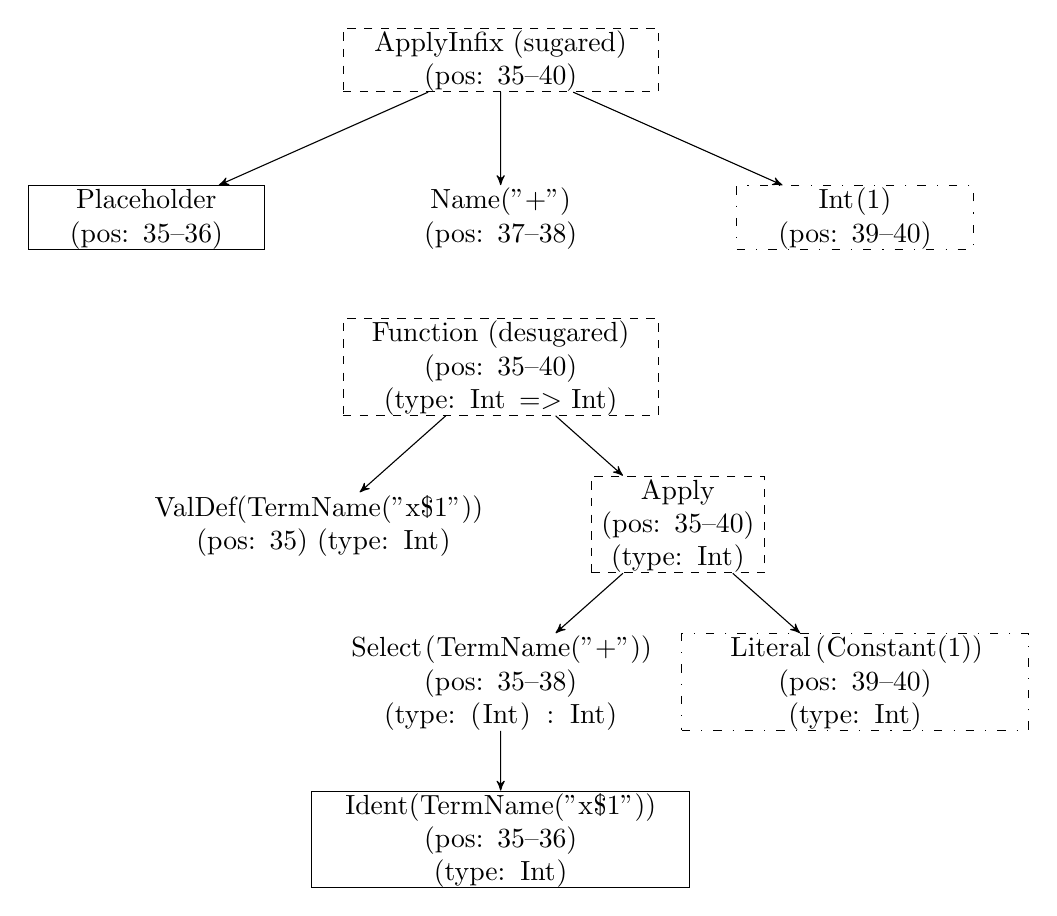
\begin{tikzpicture}[->,>=stealth',level/.style={sibling distance = 4.5cm,
  level distance = 2cm, text width=4.5cm}]
  \node (a) [draw, dashed, text width=4cm]{$\strut$ \lstinline|ApplyInfix| (sugared)
    $\strut$ \\ (pos: 35--40)
   }
    child{ node [draw, text width = 3cm]
         {$\strut$\lstinline|Placeholder| \\ (pos: 35--36)}}
      child{ node (plus) {$\strut$ \lstinline|Name("+")| $\strut$ \\
        (pos: 37--38)}}
      child{ node [text width = 3cm, draw, loosely dash dot] {$\strut$ \lstinline|Int(1)| $\strut$ \\ 
          (pos: 39--40)}};

    \node (b) [below of = plus, yshift = -0.9cm, text width=4cm, draw, dashed]
      {$\strut$ \lstinline|Function| (desugared) $\strut$ \\
         (pos: 35--40) (type: \lstinline|Int => Int|)
      }
      child{ node [text width=5cm]
           {$\strut$\lstinline|ValDef(TermName("x$1"))| $\strut$ \\
             (pos: 35) (type: \lstinline|Int|)}
         }
      child{ node [text width = 2.2cm, draw, dashed] (getter) {$\strut$\lstinline|Apply|$\strut$ \\
          (pos: 35--40) \\ (type: \lstinline|Int|)}
        child { node {$\strut$\lstinline|Select(TermName("+"))|$\strut$ \\
            (pos: 35--38) \\
            (type: \lstinline|(Int) : Int|)}
          child { node [text width = 4.8cm, draw]
            {$\strut$\lstinline|Ident(TermName("x$1"))|$\strut$ \\
              (pos: 35--36) \\ (type: \lstinline|Int|)
            } }
        }
        child { node [text width = 4.4cm, draw, loosely dash dot]
          {$\strut$\lstinline|Literal(Constant(1))|$\strut$\\
            (pos: 39--40) \\ (type: \lstinline|Int|)
          } }
      }
%%      child{ node (setter) {$\strut$ Select(TermName("+")) $\strut$ \\
%%          (pos: 30)}}
%%      child { node {$\strut$ \lstinline|Ident(TermName("x1"))| } } }
      ;
  \end{tikzpicture}
  \caption{Sugared and desugared ASTs of \lstinline|_ + 1|.
    Positions are given in offsets.}
  \label{fig:inc-asts}
\end{figure}

For the array element overwrite, we use the following program:
\begin{lstlisting}
  object O {
    def main(args : Array[String]) {
      val xs : Array[String] = Array("zero", "one", "")
      xs(2) = "two"
    }
  }
\end{lstlisting}
The sugared and desugared ASTs of the assignment @xs(2) = "two"@ is
shown on Figure~\ref{fig:array-asts}. Every node in the sugared can be
annotated since each node is in one or more same-position
relationships. The types of @Update@, @Int(2)@ and @String("two")@ are
@Unit@, @Int@, @String@, respectively. However, @Name("xs")@ receives
two distinct types: the correct type @Array[String@ and the type of
the method @update@, which is @(Int, String) : Unit@. Again, this is a
result of violation of position consistency.

\begin{figure}[t]
  \centering
  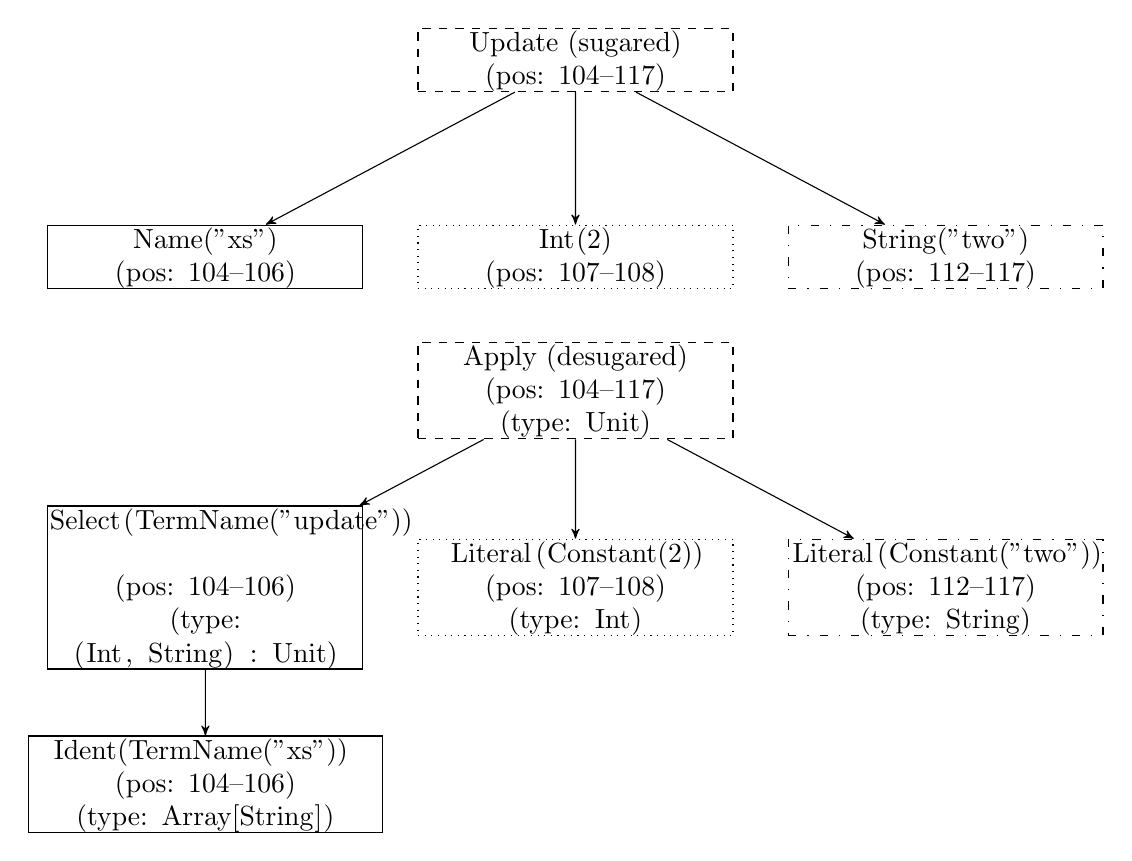
\begin{tikzpicture}[->,>=stealth',level/.style={sibling distance = 4.7cm,
  level distance = 2.5cm, text width=4cm}]
  \node (a) [text width=4cm, draw, dashed]{$\strut$ \lstinline|Update| (sugared)
    $\strut$ \\ (pos: 104--117)
   }
    child{ node [draw]
         {$\strut$\lstinline|Name("xs")| \\ (pos: 104--106)}}
      child{ node [draw, dotted] (int) {$\strut$ \lstinline|Int(2)| $\strut$ \\
        (pos: 107--108)}}
      child{ node [draw, loosely dash dot] {$\strut$ \lstinline|String("two")| $\strut$ \\ 
          (pos: 112--117)}};

    \node (b) [below of = int, yshift = -0.7cm, text width=4cm, draw, dashed]
      {$\strut$ \lstinline|Apply| (desugared) $\strut$ \\
         (pos: 104--117) (type: \lstinline|Unit|)
      }
      child{ node [draw]
           {$\strut$\lstinline|Select(TermName("update"))| $\strut$ \\
             (pos: 104--106) \\ (type: \lstinline|(Int, String) : Unit|)}
           child {
             node [text width = 4.5cm, draw] {$\strut$\lstinline|Ident(TermName("xs"))| $\strut$ \\
               (pos: 104--106) \\
               (type: \lstinline|Array[String]|)}
             }
         }
      child{ node [draw, dotted] (getter) {$\strut$\lstinline|Literal(Constant(2))|$\strut$ \\
          (pos: 107--108) \\ (type: \lstinline|Int|)}
        }
      child { node [draw, loosely dash dot] {$\strut$\lstinline|Literal(Constant("two"))|$\strut$ \\
            (pos: 112--117) \\
            (type: \lstinline|String|)}
        }
      ;
  \end{tikzpicture}
  \caption{Sugared and desugared ASTs of \lstinline|xs(2) = "two"|.
    Positions are given in offsets.}
  \label{fig:array-asts}
\end{figure}

\section{Evaluation}
\label{sec:eval}

The problem to be solved is implementation of a suitable front end for
a variety of external language processing tools. Most common features
that these tools offer are \emph{static analysis} and \emph{program
  code transformation}. Many tools statically analyse the code at
hand, and even perform transformation based on information from static
analysis, combining the two features. We elaborate on the effect of
hybrid front ends on these features in what follows.

\subsection{Benefits in program code transformation}

External tools which perform source code transformations would
benefit from a front end that generates a more accurate source code
representation. A typical workflow consists of parsing, locating the
code to be transformed in the AST, transformation and pretty printing
the AST.

A hybrid front end may improve locating the code in the AST in
specific cases. Depending on the compiler front end infrastructure and
the order and organisation of the compilation phases, the AST may
become subject to optimizations and compile time meta-programming. By
the time the external tool receives the AST, constant expressions may
be folded, and meta-programming constructs are expanded into generated
code. It may happen that the programmer specifies a (part of a)
meta-programming construct as the subject of a code transformation,
and the compiler front end replaces it with its expansion in the AST,
thus the search in the AST fails.

Benefit in pretty printing is clear. A hybrid front end retains
lexical and syntactical information on the code. The retained
information, which includes syntactic sugars, comments and
whitespaces, helps the pretty printer to generate code that pleases
the programmer. Without this information, as a side effect,
@for@-loops may become @foreach@ functions, invaluable documentation
comments may be lost, and tabs may be replaced with spaces or vice
versa, throwing away careful indentation.

\subsection{Effect on static analysis}

% grokking, jump-to-definition vs macros
% interprocedurális elemzések, lásd Assign

The difference between ASTs in representation of the same statement,
such as the assignment @counter = counter + 1@, may cause ambiguity in
interprocedural semantic analyses. This statement can be regarded as
an assignment, where the value from the right hand side flows to the
left hand side, or as an invocation of the setter method @counter_=@
in the class @Counter@.

We can resolve this ambiguity in the following way. When the user does
not define a setter for @counter@, the compiler will generate a
trivial setter. In that case, the analysis can treat the statement as
an assignment. Otherwise, the assignment regarded as an invocation of
the setter method.

\section{Related work}
\label{sec:related}
Several programming languages offer syntactic sugars to make software
development more convenient and efficient. At first, we would like to present a
resugaring technique in Scala, and then investigate other languages as
well.

\subsection{Resugaring in Scala}

An alternative approach to build a language processing tool is to
further enhance the annotated AST provided by an external tool by
undoing the desugaring and adding the sugared syntax tree to the
representation. In~\cite{sclit17} we introduced a \emph{resugaring} algorithm
for Scala by linking two ASTs, a sugared and a desugared,
together. The output is a joint AST which includes terminal and
non-terminal nodes of both ASTs and the links between them.
Figure~\ref{fig:joint-ast} illustrates the relevant fragment of the
joint AST of the @Counter@ class, with a sugared AST constructed with
Scalameta, and a desugared AST provided by the \emph{scalac} compiler.

\begin{figure}[!htb]
  \centering
  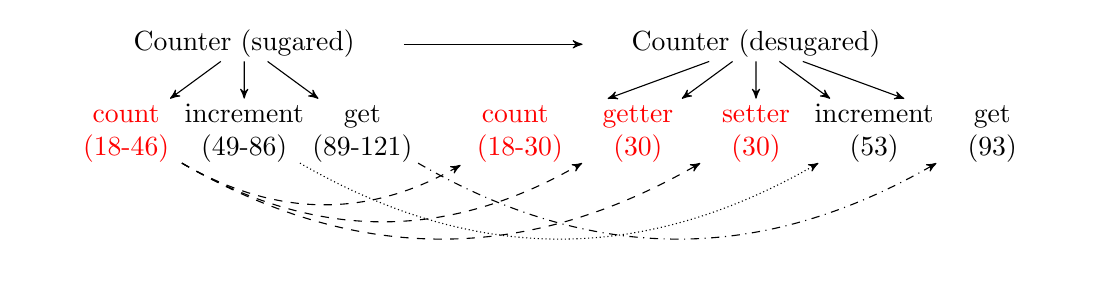
\begin{tikzpicture}[->,>=stealth',level/.style={sibling distance = 1.5cm,
  level distance = 1.1cm, text width=2.5cm}]
    \node (a) {$\strut$ \lstinline|Counter| (sugared) $\strut$}
    child{ node (count-left) [highlight] 
         {$\strut$\lstset{identifierstyle=\color{red}}\lstinline|count| \\
        \color{red} (18-46)}}
      child{ node (inc-left) {$\strut$ \lstinline|increment| $\strut$ \\
        (49-86)}}
      child{ node (get-left) {$\strut$ \lstinline|get| $\strut$ \\ 
        (89-121)}}
    ;
    \node (b) [right of = a, xshift = 5.5cm] 
        {$\strut$ \lstinline|Counter| (desugared) $\strut$}
      child{ node (count-right) [highlight] 
           {$\strut$\lstset{identifierstyle=\color{red}}\lstinline|count| $\strut$ \\ \color{red} (18-30)} }
      child{ node (getter) [highlight] {$\strut$ getter $\strut$ \\
          (30)} }
      child{ node (setter) [highlight] {$\strut$ setter $\strut$ \\
          (30)} }
      child{ node (inc-right) {$\strut$ \lstinline|increment| $\strut$ \\
          (53)}}
      child{ node (get-right) {$\strut$ \lstinline|get| $\strut$ \\
          (93)}}
      ;
    \draw [shorten >= 0.5cm, shorten <= 0.5cm] (a) edge (b);
    \draw [bend right, dashed, shorten >= 0.05cm] (count-left) edge (count-right);
    \draw [bend right, dashed] (count-left) edge (getter);
    \draw [bend right, dashed] (count-left) edge (setter);
    \draw [bend right, densely dotted] (inc-left) edge (inc-right);
    \draw [bend right, dash dot] (get-left) edge (get-right);
  \end{tikzpicture}
  \caption{Resugared AST of the \lstinline|Counter| class. Positions
    are given in offsets.}
  \label{fig:joint-ast}
\end{figure}

%% We can establish connection between nodes of the two ASTs using
%% position information. Let us assume that both terminal and
%% non-terminal nodes have information about its position in the source
%% file. Position ranges of non-terminal nodes are synthesized from the
%% positions of their children. Now we can conclude that two nodes are
%% related if they are roots of subtrees of the same code fragment, that
%% is, position information of their tokens overlap. It is a peculiarity
%% of parser implementation that we cannot check for equality of
%% positions, since the two parsers might handle position ranges
%% differently, as Figure~\ref{fig:joint-ast} shows.

The links between
the nodes of the two ASTs are established by an algorithm that
traverses the two ASTs simultaneously in level-order.
The algorithm is presented on Figure~\ref{fig:res}.
%Due to space
%limits, we present the algorithm here without further explanation.

\begin{figure}[!htb]
\begin{lstlisting}[mathescape=true,escapechar=\`,deletekeywords={with}]
  `\textsc{Resugar}`($tree_s$, $tree_d$)
    let $tree_s$ be the root of sugared and $tree_d$ the root of the
      desugared AST
    $edges$ = `\textsc{Resugar-Children}`($tree_s$, $tree_d$)
    if `\textsc{Position}`($tree_s$) overlaps `\textsc{Position}`($tree_d$)
      `\textsc{Add}`($edges$, `\textsc{Edge}`($tree_s$, $tree_d$))
    return $edges$

  `\textsc{Resugar-Children}`($tree_s$, $tree_d$)
    let $edges$ be an empty set of links between the nodes
    let $mapping$ be an empty mapping from positions to nodes
    for $i$ = 1 to `\textsc{Num-Children}`($tree_d$)
      `\textsc{Add}`($mapping$,
          `\textsc{Position}`(`\textsc{Children}`($tree_d$, $i$)),
          `\textsc{Children}`($tree_d$, $i$))
    for $i$ = 1 to `\textsc{Num-Children}`($tree_s$)
      if `\textsc{Children}`($tree_s$, $i$) has a matching node in $mapping$
        let $match$ be the desugared node with overlapping
          position in $mapping$
        `\textsc{Union}`($edges$,
              `\textsc{Resugar-Children}`(`\textsc{Children}`($tree_s$, $i$), $match$))
        return $edges$
\end{lstlisting}
\caption{Resugaring algorithm}
\label{fig:res}
\end{figure}
\subsection{Syntactic sugars in other languages}

The records in Erlang are taken as syntactic sugar, thus are
translated to tuple expressions by the compiler. A record of
\textit{n} fields is substituted with a tuple of \texttt{n+1}
elements, where the very first element is the name of the record and
the following elements are the values of the fields (listed in the
defined field order).

There are two major refactoring tools for Erlang,
RefactorErl~\cite{kept09} and Wrangler. These tools use different
approaches in source code processing. RefactorErl follows a standalone approach: it uses its own
analyser framework to make every bit of information available. Even
the layout, comment, preprocessor constructs and record information are
stored in the Semantic Program Graph (SPG), thus the source code
restoration with its context is straightforward. Opposed to
RefactorErl, the Wrangler tool~\cite{wrangler} is closer to the external approach,
since it uses the standard \emph{syntax tools}~\cite{erlsyntax} library that
comes with Erlang OTP. Atop of the standard parser, however, the
tool annotates the AST with additional information with macro, record
and layout information.

The Glasgow Haskell Compiler ~\cite{aosaghc} uses several well
separated phases in the compilation process. The type checking is
performed right before the desugaring phase, thus extracting the
representation after the type checking phase includes information on
syntactic sugar constructs. The Haskell-tools~\cite{haskelltools}
refactoring framework uses this representation for further analysis and
transformation -- this is an external approach.

\subsection{Preprocessor constructs}
Preprocessor constructs, such as macros, can also be considered as a
special form of desugaring. In the original source code a macro
application is presented, but usually well before the static semantic
analysis a preprocessor substitutes the macro application with the
corresponding macro body, and the compiler builds the annotated AST
from the expanded macro body. This raises a similar problem as the
desugaring in a language processing tool. For example, the source code
needs to be pretty printed after a refactoring transformation with 
the original macro applications kept.

For Erlang, the tool RefactorErl provides a custom
parser to store both the original code and the
preprocessed one~\cite{kitlei,erlws10}. This makes the pretty printing after refactoring
straightforward, and the static analysis more accurate on the expanded
AST.

The C programming language also provides a powerful macro system. The
tool CRefactory~\cite{cpreproc} introduces a standalone approach to
solve the same issue by preserving the preprocessor directives during parsing.

%\paragraph{Refactoring preprocessor constructs in C}
%\paragraph{Static analysis of preprocessor constructs in Erlang}


\section{Conclusion}
\label{sec:concl}
In this paper, we elaborated on how to implement a programming
language processing tool in order to minimize the effort. We showed
that building upon modern compiler infrastructure helps, but it comes
at the price of losing information, due to desugaring. We presented
an approach, \emph{front end fusion}, to circumvent this. We proposed
an algorithm to construct an annotated abstract syntax tree by fusing
the ASTs of the Scala compiler and the Scalameta library.

The presented algorithm is based on the simultaneous traversing of the
ASTs to be fused while considering the position consistency of the
desugared nodes. We also discussed the need of type-preserving
desugaring in terms of the fusion, and presented the solution for the
Scala-specific deviations.

%%The paper discusses the advantages of our approach in language
%%processing tools.

We have implemented and evaluated our methodology by creating a
language processing tool for Scala with the aim of providing a
refactoring framework for parallelisation. However the presented
approach can be used for other programming languages as well, where
the required compiler front end is easily accessible.

%There are still many open issues for future research. Code
%transformations on resugared AST requires the overhead of keeping two
%ASTs synchronized. This needs to be implemented without overly
%complicating code transformations.

\newpage

\bibliographystyle{plain}%
\bibliography{biblio}%

\end{document}
